\chapter{HOPG-Probe}
%Bevor die HOPG-Probe mit atomarer Auflösung analysiert werden kann, wird ihre grobe Oberflächenstruktur zunächst mit einem USB-Lichtmikroskop untersucht. Abbildung !!!ADDREF!!!! zeigt den Zustand der Probe (HOPG) nach dem Entfernen einer Schicht. Es ist zu erkennen, dass die oberste Graphitschicht keine gleichmäßig ebene Oberfläche aufweist, sondern aus mehreren plattenartigen Segmenten besteht, die in unterschiedlichen Winkeln zueinander ausgerichtet sind. Dies wird durch die unterschiedlichen Reflexionswinkel der einzelnen Bereiche deutlich.

%Um eine möglichst glatte Oberfläche für die Analyse mit einem Rastertunnelmikroskop zu erzeugen, wird die oberste Graphitschicht erneut mit Klebeband entfernt. Nach dieser Behandlung erscheint die Probe optisch glatt, das mit dem USB-Mikroskop aufgenommene Bild !!!!ADDREF!!! zeigt jedoch noch eine gewisse Segmentierung (!!!!!CONFIRM OR NOT THIS OBSERVATION!!!!). Für RTM-Untersuchungen ist jedoch nur eine ebene Oberfläche über wenige Quadratnanometer erforderlich, sodass der hergestellte Zustand als ausreichend geeignet gilt.

%Im nächsten Schritt wird die HOPG-Probe in den Probenhalter des Rastertunnelmikroskops eingesetzt. Zusätzlich wird eine neue Spitze für die Untersuchung vorbereitet und in die dafür vorgesehene Klemme des STM eingesetzt. Eine vergrößerte Abbildung der Spitze ist in Abbildung !!!!ADDREF!!! dargestellt.


%Nach erfolgreicher Positionierung von Probe und Spitze erfolgt die Annäherung zunächst mit "advance" und anschließend mit "approach". Sobald die Steuerelektronik den Tunnelkontakt registriert, kann die Messung gestartet werden. Es wurden mehrere Bilder mit unterschiedlichen Vergrößerungen aufgenommen.

%Das RTM wurde zunächst im "Constant Current Mode" betrieben, um Kollisionen der Spitze mit möglichen Oberflächenunebenheiten zu vermeiden. Der "Constant Height Mode" wurde später für hochauflösende Detailbilder auf atomarer Ebene verwendet.

%Abbildung !!!ADDREF!!! zeigt ein Bild einer Graphitoberfläche mit einem Raster von !!!ADDSCALING!!! Kantenlänge. Da es im "Constant Current Mode" aufgenommen wurde, enthält das Höhenbild !!!WHERE!!! topografische Informationen. Der dargestellte Ausschnitt zeigt drei weitgehend planare Segmente der Graphitoberfläche, die bereits im Lichtmikroskopbild makroskopisch sichtbar waren !!!ADDREF!!!. Ihre Kanten sind scharf, was im Strombild !!!WHERE!!! besonders deutlich wird, da der PID-Regler eine schnelle Änderung des Tunnelstroms erfasste. Insgesamt zeigt das Strombild, dass der Regelkreis einen weitgehend konstanten Tunnelstrom aufrechterhält, was auf eine präzise Einstellung der Regelparameter hindeutet. !!!CONFIRM/DENYOBSERVATION!!!

%Das Höhenbild in !!!ADDREF!!! zeigt deutlich, dass der zu beobachtende Probenbereich für die atomare Auflösung geeignet ist, da das zentrale Segment eine nahezu flache Struktur im Nanometerbereich aufweist.!!!CONFIRM/DENYOBSERVATION!!! 

%Zur Bestätigung !!!DIDWEDOTHAT???!!!!!! wurde zusätzlich ein kleineres Ausschnittsbild von !!!!ADDSCALING!!! aufgenommen. Das Ergebnis dieser Messung ist in !!!!ADDREF!!!! dargestellt.

%Es gibt keine größeren Unregelmäßigkeiten im gescannten Gebiet. Lediglich vereinzelte Abweichungen vom Mittelwert sind sowohl im Höhenbild als auch im Strömungsbild erkennbar. Zur quantitativen Analyse ist die Verteilungsfunktion der Höhenwerte in !!!ADDREF-HÖHENPROFIL!!! dargestellt. Die Daten können durch eine Gauß-Funktion mit Mittelwert !!!!!!!!!!ADD-PARAMETERS-GAUSSFIT mu =  und Standardabweichung sigma= !!!!!!!!!!!! modelliert werden.

%Da der Bereich \( \sigma \) sehr klein ist, kann angenommen werden, dass die Aufnahme im "Constant Height Mode" durchgeführt werden kann, ohne die Spitze oder die Probe zu beschädigen. Um in diesen Modus zu wechseln, wird der PID-Regler mit den Parametern P = 0, I = 4, D = 0 eingestellt.

%Die nächste Aufnahme wird mit einer Scanbreite von !!!!ADDSCALE!!!!!! durchgeführt. Abbildung !!!!ADDREF!!!!! zeigt die entsprechenden Messergebnisse des RTM. Da in dieser Aufnahme der "Constant Height Mode" verwendet wurde, enthält das aktuelle Bild nun topografische Informationen. Das Höhenbild zeigt nur Stellen, an denen die feste Komponente des PID-Reglers kleine Höhenanpassungen vorgenommen hat, um große Bodenunebenheiten oder Gefälle.

%!!!!ADD PICS AND COMMENTS EXPLAINING THAT YOU CAN'T SEE SHIT AND MAYBE SOME PICS OF WHAT IT SHOULD LOOK LIKE THEORETICALLY AND HOW WE WOULD DETERMINE THE ANGLE AND THE DISTANCE WITH GOOD PICS!!!!!!

Nach der Einarbeitung in den Betrieb des STM am Goldmuster wurde nun der Graphitprobe Aufmerksamkeit geschenkt. Diese Probe besteht aus hochorientiertem pyrolytischem Graphit (HOPG). Die Kristallstruktur dieser Probe ist schematisch in \cref{fig:HOPG_struktur} dargestellt. 
\begin{figure}[H]
    \centering
    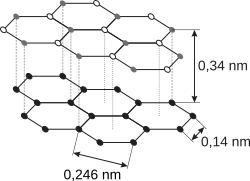
\includegraphics[width=0.75\textwidth]{figs/Hpg_struktur.png}
    \caption{Zwei übereinander gestapelte Schichten von Graphit (HOPG), die die hexagonale Anordnung der Kohlenstoffatome zeigen. Schwarze Punkte markieren Atome, die direkt über einem Atom in der darunterliegenden Schicht sitzen, weiße Punkte solche, die dies nicht tun. 
    Die C-C-Bindung in der Ebene beträgt $\SI{0.14}{\nano\metre}$, die Gitterkonstante ist $\SI{0.246}{\nano\metre}$ und der Schichtabstand beträgt $\SI{0.34}{\nano\metre}$.  \cite{praktikum}}
    \label{fig:HOPG_struktur}
\end{figure} 

Die Abstände zwischen benachbarten Schichten sowie zwischen benachbarten Atomen innerhalb derselben Schicht sind angegeben. Die einzelnen Kohlenstoffatome in einer Lage sind über kovalente Bindungen stark miteinander verbunden, während die verschiedenen Lagen durch schwächere van-der-Waals-Wechselwirkungen zusammengehalten werden. 
Dies wird auch in \cref{fig:HOPG_struktur} durch die unterschiedlichen Größenordnungen der Schicht- und Atomabstände deutlich. Praktisch bedeutet dies, dass sich die einzelnen Graphitschichten leicht voneinander trennen lassen.


Es ist ebenfalls ersichtlich, dass benachbarte Schichten gegeneinander versetzt sind, sodass die Hälfte aller Kohlenstoffatome keinen direkten Nachbarn in der darunterliegenden Schicht besitzt (siehe \cref{fig:HOPG_struktur}). Diese Tatsache spielt eine bedeutende Rolle bei der späteren Beobachtung mittels STM.
Die Elektronendichte eines Atoms hängt von dessen umgebenden Nachbarn ab; Kohlenstoffatome ohne direkte Nachbarn in der darunterliegenden Schicht, als B-Atome gekennzeichnet, weisen in ihrer Umgebung eine leicht erhöhte Elektronendichte auf. 
Dementsprechend werden sie am klarsten aufgelöst und erscheinen als Maxima der Elektronendichte. 

Atome der unteren Schicht, die sich im Zentrum der oberen Schicht befinden und als H-Atome bezeichnet werden, können aufgrund des großen Abstands zwischen den Schichten nicht aufgelöst werden und erscheinen als Minima in der Elektronendichte. 
Atome mit Nachbarn in der darunterliegenden Schicht, als A-Atome gekennzeichnet, könnten theoretisch aufgelöst werden, sind jedoch in der Topographie der Elektronendichte nicht sichtbar. 
Dies liegt daran, dass die Elektronen des benachbarten Atoms in der unteren Schicht die Elektronen des A-Atoms abstoßen und so deren Dichte um das A-Atom herum ausbreiten; die Intensitätsverteilung der Elektronendichte des A-Atoms wird verzerrt - ihre Amplitude nimmt ab und ihre Breite zu.


Für die Durchführung der Messung wird analog zur Abbildung der Goldprobe vorgegangen. 
Die Oberfläche des Probenhalters und die Unterseite der Graphitprobe werden mit Isopropanol gereinigt.
Die Oberfläche der Graphitprobe wird mittels Klebeband abgezogen, um Staub und Verunreinigungen zu entfernen. Aufgrund der schwachen Wechselwirkungen zwischen den Schichten ist dies leicht realisierbar. 
In \cref{fig:graphene} sind die beiden USB-Mikroskopbilder der Graphitoberfläche vor und nach dem Abziehen dargestellt.

\begin{figure}[H]
    \centering
    \begin{minipage}[t]{0.495\textwidth}
        \centering
        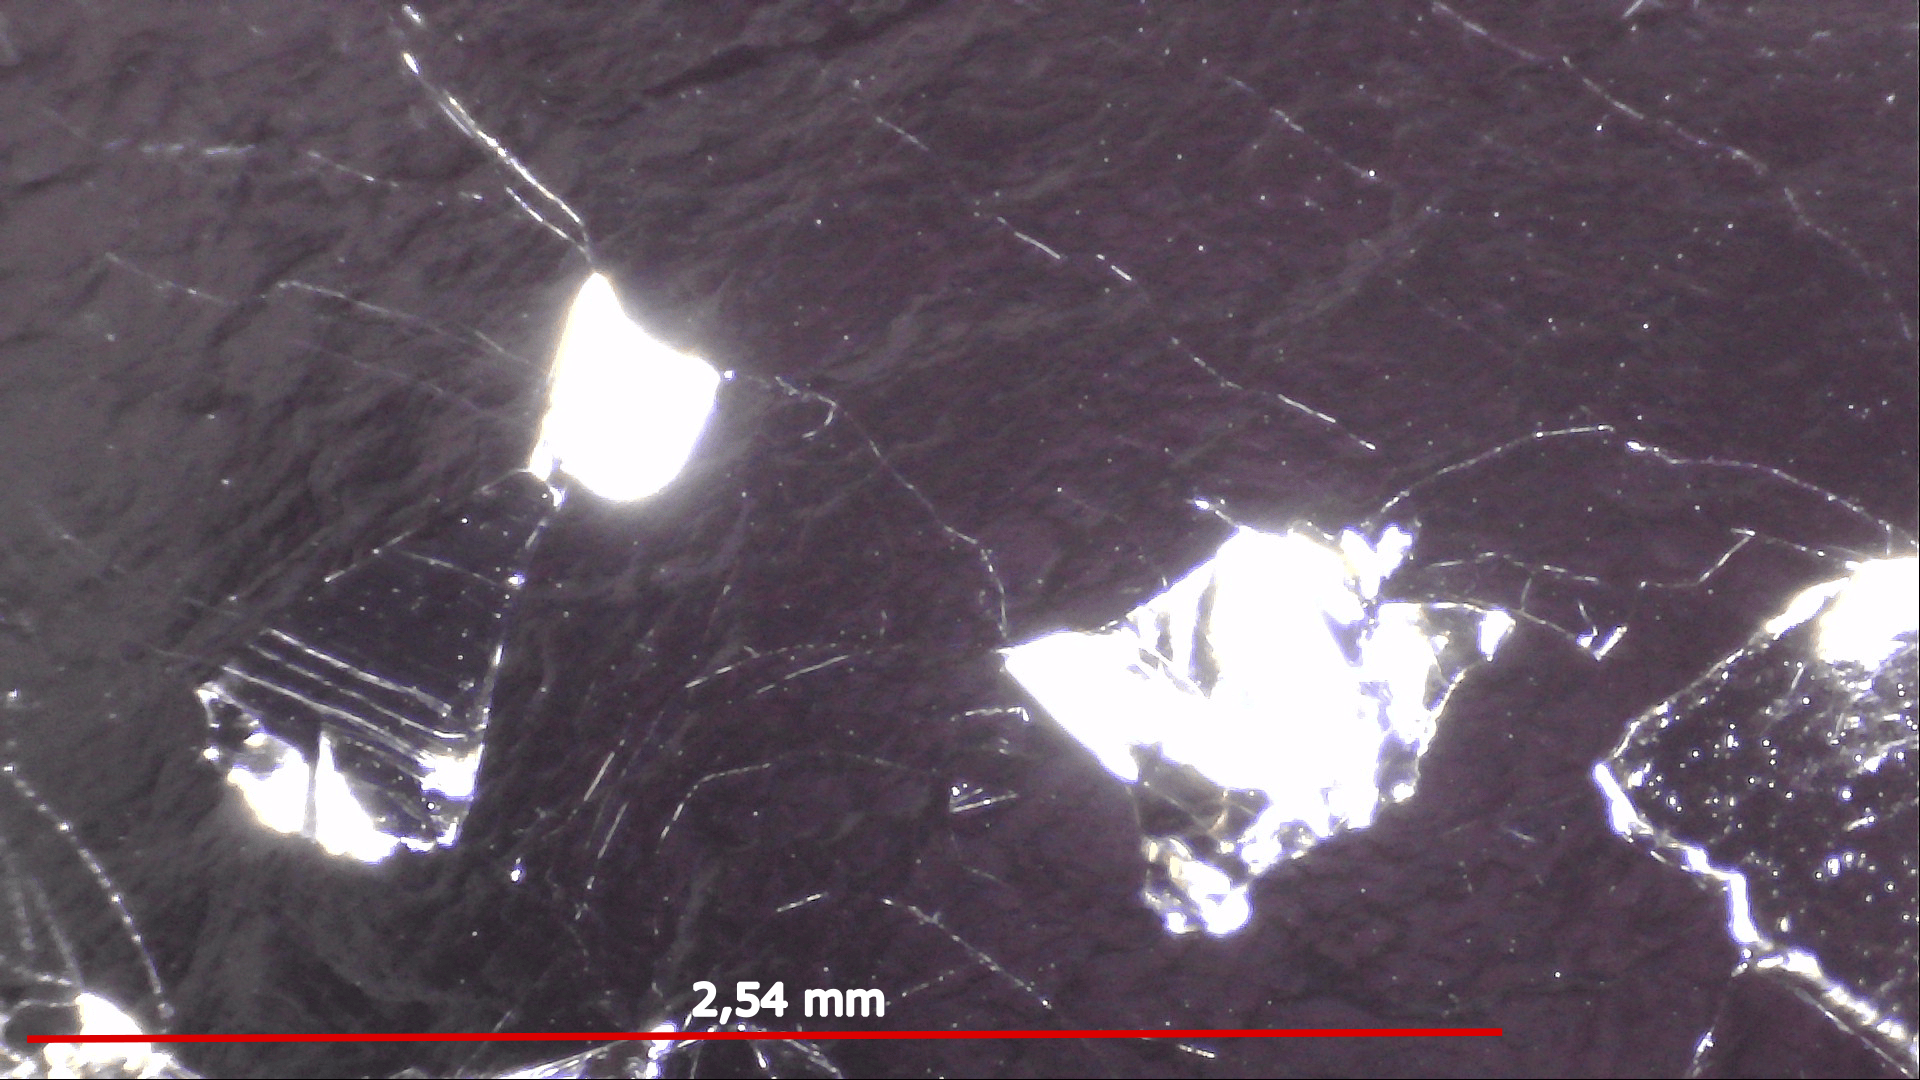
\includegraphics[width=\textwidth]{editgraphite17_before.png}
        \subcaption{vor Abziehen der Oberfläche}
        \label{fig:graphenea}
    \end{minipage}
    \hfill
    \begin{minipage}[t]{0.495\textwidth}
        \centering
        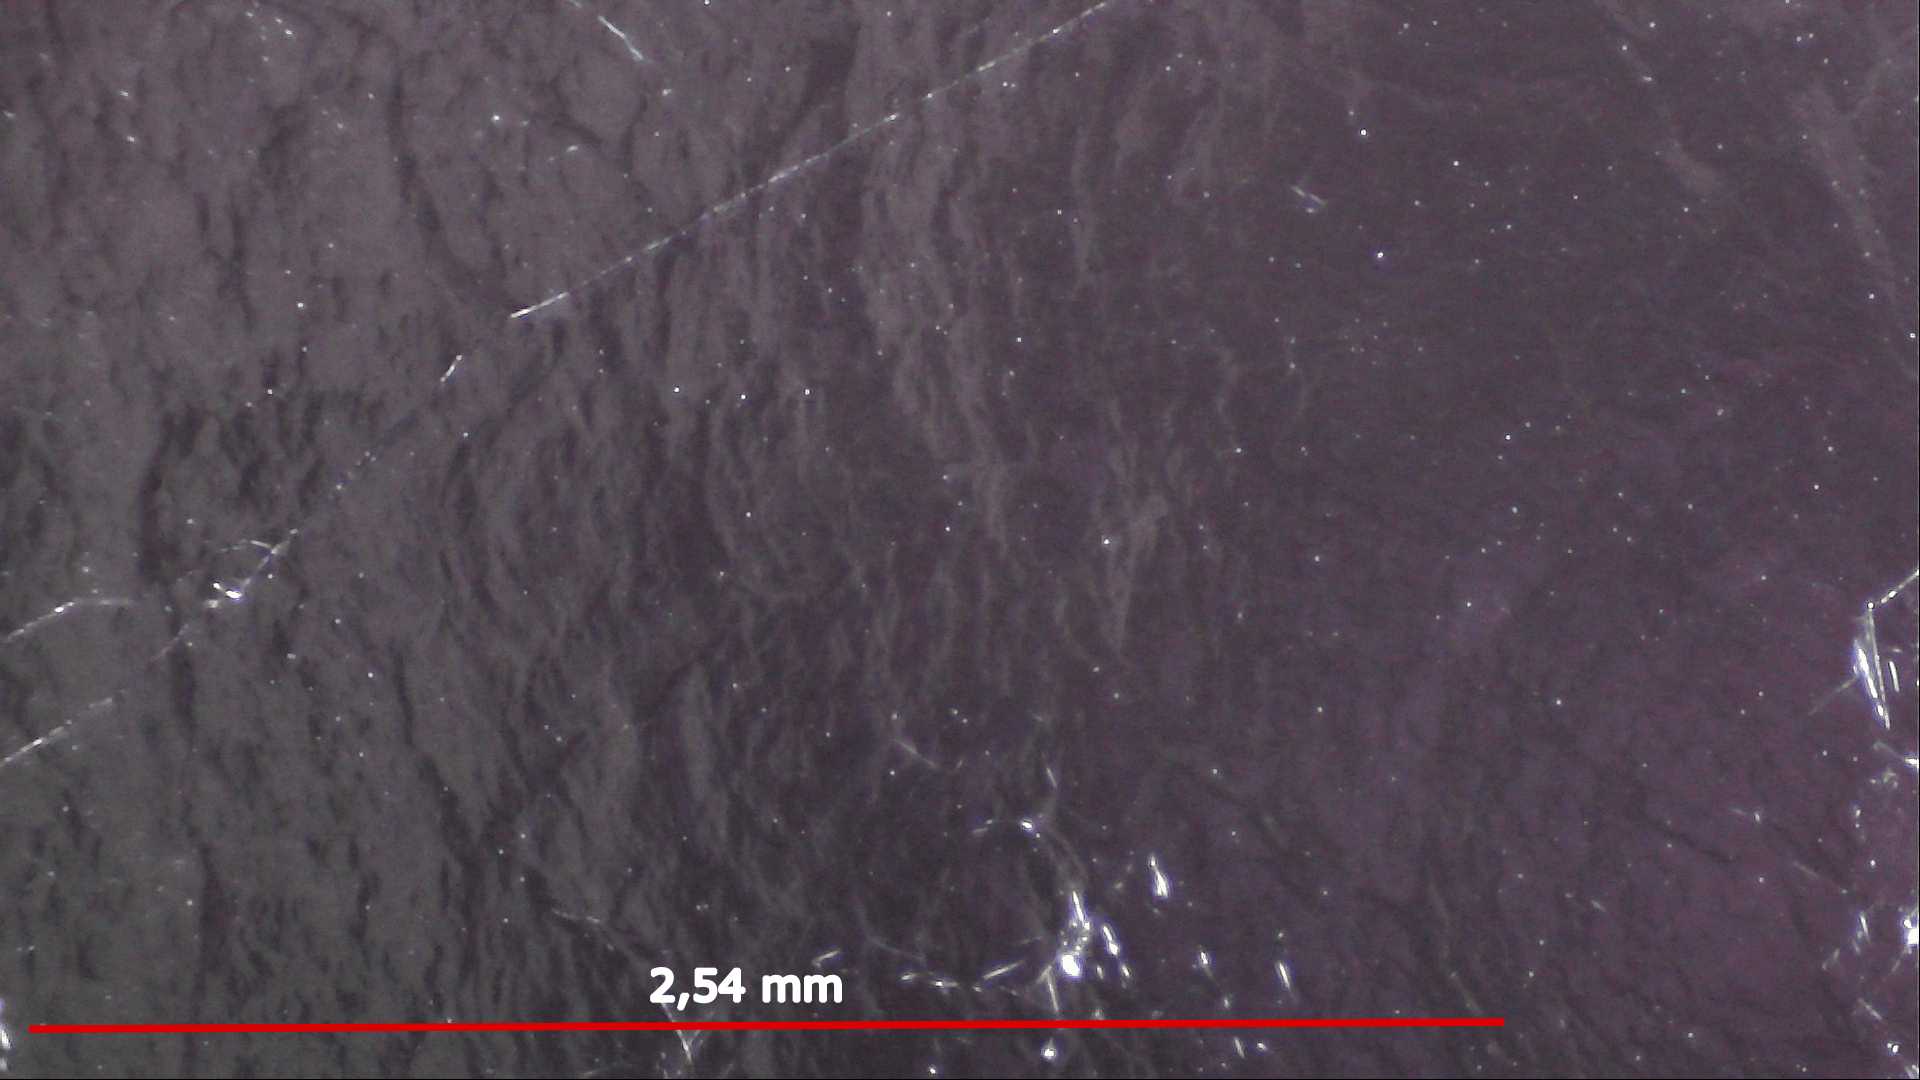
\includegraphics[width=\textwidth]{editgraphite_after_waxing.png}
        \subcaption{nach Abziehen der Oberfläche}
        \label{fig:grapheneb}
    \end{minipage}
    \caption{
      Aufnahmen der Graphitoberflächen mit der USB-Lupe vor und nach Aufziehen der Oberfläche mit dem Klebeband mit einer Linie der Länge $\SI{2.54}{\mm}$ als Maßstab.
}
    \label{fig:graphene}
\end{figure}

Um die atomare Struktur zu messen, wurde zunächst ein großer Bereich von $\SI{200}{\nm} \times \SI{200}{\nm}$ gescannt, um eine möglichst ebene Region zu finden. 
Diese Messung musste mehrfach wiederholt werden, da die Graphitoberfläche hochgradig unregelmäßige Strukturen aufwies, die sogar makroskopisch in \cref{fig:graphene} sichtbar sind. 
Infolgedessen kam die Spitze während des Scans häufig mit der Oberfläche in Kontakt, was zu wiederholtem Nachschärfen der Spitze führte. 

Schließlich wurde durch Drehen der Probe eine ebene Fläche gefunden, auf der der Scan durchgeführt werden konnte. Das Ergebnis ist in \cref{fig:hopg_good} dargestellt. 

\begin{figure}[H]
    \centering
    \begin{minipage}[t]{0.495\textwidth}
        \centering
        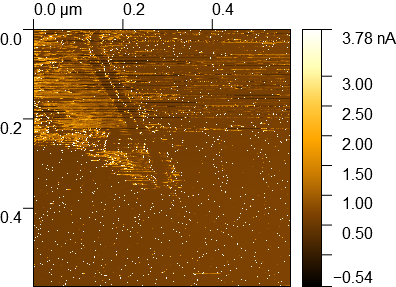
\includegraphics[width=\textwidth]{graphit_theonewithgoodzvaluesI.png}
        %\label{fig:g_good_I}
    \end{minipage}
    \hfill
    \begin{minipage}[t]{0.495\textwidth}
        \centering
        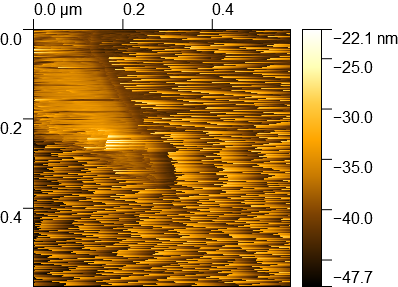
\includegraphics[width=\textwidth]{graphit_theonewithgoodzvaluesZ.png}
        %\label{fig:g_good_Z}
    \end{minipage}
    \caption{
      RTM-Aufnahme HOPG $\SI{575}{\nm}$; links: Tunnelstrom, rechts: Z-Achse; Setpoint $I = \SI{1}{\nano\ampere}$, Tip voltage $U = \SI{450}{\milli\volt}$,Rastergeschwindigkeit $v = \SI{1916.7}{\nano\meter\per\second}$; $P = 1000$, $I = 2000$, $D = 0$
}
    \label{fig:hopg_good}
\end{figure}

Die raue und unregelmäßige Struktur ist in dieser Abbildung ebenfalls deutlich erkennbar. Die Farbskala hebt die sehr große Variation in der Höhe der Spitze über der Probe hervor, die sich über einen Bereich von $\SI{25.6}{\nm}$ erstreckt. 
Der obere linke Bereich des Areals zeigt eine relativ homogene Struktur und wird daher genauer untersucht. In dieser Ecke wird über ein Gebiet von $\SI{10}{\nm} \times \SI{10}{\nm}$ gescannt. Das Ergebnis ist in \cref{fig:10nmCC} und \cref{fig:10nmCH} zu sehen.

\begin{figure}[H]
    \centering
    \begin{minipage}[t]{0.495\textwidth}
        \centering
        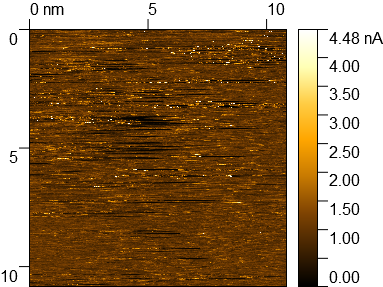
\includegraphics[width=\textwidth]{graphit_constant_current_10nm_I.png}
        %\label{fig:g_good_I}
    \end{minipage}
    \hfill
    \begin{minipage}[t]{0.495\textwidth}
        \centering
        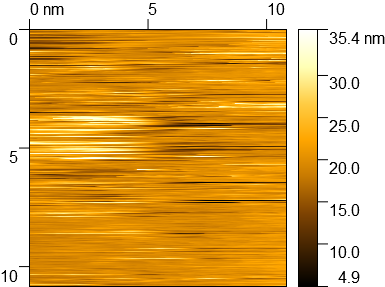
\includegraphics[width=\textwidth]{graphit_constant_current_10nm_Z.png}
        %\label{fig:g_good_Z}
    \end{minipage}
    \caption{
      RTM-Aufnahme HOPG $\SI{10.8}{\nm}$; links: Tunnelstrom, rechts: Z-Achse; Setpoint $I = \SI{1}{\nano\ampere}$, Tip voltage $U = \SI{450}{\milli\volt}$,Rastergeschwindigkeit $v = \SI{35.6}{\nano\meter\per\second}$; $P = 1000$, $I = 2000$, $D = 0$
}
    \label{fig:10nmCC}
\end{figure}

\begin{figure}[H]
    \centering
    \begin{minipage}[t]{0.495\textwidth}
        \centering
        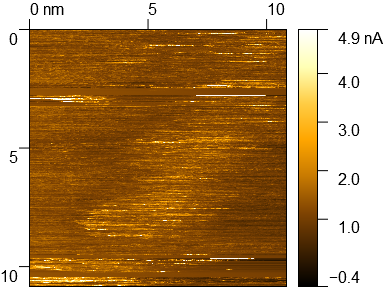
\includegraphics[width=\textwidth]{graphit_constant_height_10nm_I.png}
        %\label{fig:g_good_I}
    \end{minipage}
    \hfill
    \begin{minipage}[t]{0.495\textwidth}
        \centering
        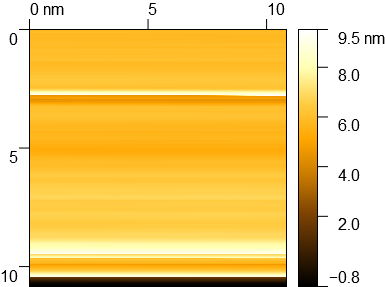
\includegraphics[width=\textwidth]{graphit_constant_height_10nm_Z.png}
        %\label{fig:g_good_Z}
    \end{minipage}
    \caption{
      RTM-Aufnahme HOPG $\SI{10.8}{\nm}$; links: Tunnelstrom, rechts: Z-Achse; Setpoint $I = \SI{1}{\nano\ampere}$, Tip voltage $U = \SI{450}{\milli\volt}$,Rastergeschwindigkeit $v = \SI{35.6}{\nano\meter\per\second}$; $P = 0$, $I = 4$, $D = 0$
}
    \label{fig:10nmCH}
\end{figure}
Aus dem in \cref{fig:10nmCH} dargestellten $\SI{10}{\nm} \times \SI{10}{\nm}$-Bereich wurde der unterer mittlerer Teil der Abschnitt für eine weitere Analyse ausgewählt. 
Dieser Bereich erscheint für eine atomare Auflösung geeignet, da nur wenige Unregelmäßigkeiten erkennbar sind, insbesondere auf der rechten Seite. Natürlich kann die atomare Struktur nicht direkt über die Messung der Spitzenhöhe über der Probe ermittelt werden. 
In \cref{fig:10nmCH} ist die Strommessung dargestellt. Wie erwartet bleibt der Strom weitgehend konstant. 
Allerdings sind einige auffällige Maxima vorhanden, die auf die endliche Reaktionszeit des Regelsystems oder auf Schwankungen zwischen Spitze und Probe zurückgeführt werden können. 
Diese Schwankungen könnten beispielsweise durch Luftzug, Bewegungen infolge von Kontakt mit der Arbeitsfläche oder andere geringe Vibrationen im Umfeld des Versuchsaufbaus verursacht worden sein.

Aus dem in Abbildung $\SI{10}{\nm} \times \SI{10}{\nm}$ dargestellten Bereich wurde der unterer mittlerer Teil der Abschnitt für eine weitergehende Untersuchung ausgewählt. 
An dieser Stelle wurde schließlich der Scan zur atomaren Auflösung durchgeführt, wobei der Bereich auf $\SI{4}{\nm} \times \SI{4}{\nm}$ eingestellt wurde. 
Zuerst erfolgte die Messung im ''Constant Current Mode'', um erneut zu bestätigen, dass die Oberfläche glatt war. Anschließend wurde die Messung im ''Constant Height Mode'' durchgeführt, um Rückschlüsse auf die atomare Elektronendichte des Kristalls zu ziehen. Leider konnten aufgrund von Zeitmangel nur Messungen im ''Constant Current Mode'' durchgeführt werden. Die resultierenden Bilder befinden sich in \cref{fig:4nmCC}

\begin{figure}[H]
    \centering
    \begin{minipage}[t]{0.495\textwidth}
        \centering
        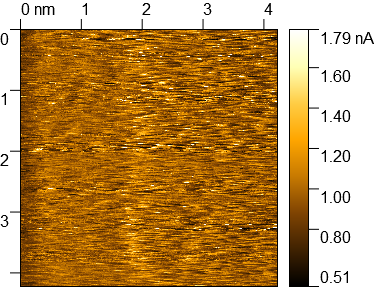
\includegraphics[width=\textwidth]{graphit_const_current_4nm_I.png}
        %\label{fig:g_good_I}
    \end{minipage}
    \hfill
    \begin{minipage}[t]{0.495\textwidth}
        \centering
        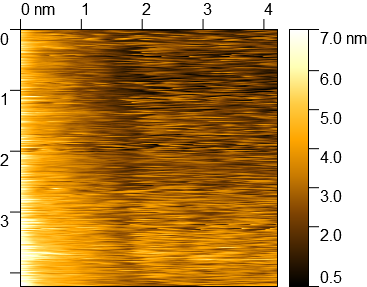
\includegraphics[width=\textwidth]{graphit_const_current_4nm_Z.png}
        %\label{fig:g_good_Z}
    \end{minipage}
    \caption{
      RTM-Aufnahme HOPG $\SI{4.22}{\nm}$; links: Tunnelstrom, rechts: Z-Achse; Setpoint $I = \SI{1}{\nano\ampere}$, Tip voltage $U = \SI{450}{\milli\volt}$,Rastergeschwindigkeit $v = \SI{13.9}{\nano\meter\per\second}$; $P = 1000$, $I = 2000$, $D = 0$
}
    \label{fig:4nmCC}
\end{figure}

Anschließend wurde, nachdem im vorherigen $\SI{4}{\nm} \times \SI{4}{\nm}$-Bereich keine Ergebnisse erzielt wurden, ein weiterer Bereich von $\SI{5}{\nm} \times \SI{5}{\nm}$ untersucht. Bilder von dieser Messung sind in \cref{fig:5nmCC} und \cref{fig:5nmCH} zu sehen.

\begin{figure}[H]
    \centering
    \begin{minipage}[t]{0.495\textwidth}
        \centering
        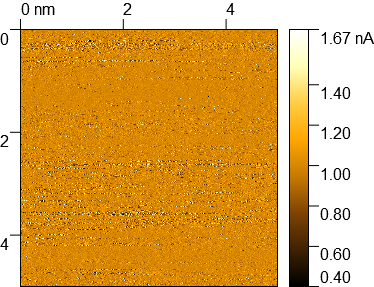
\includegraphics[width=\textwidth]{graphit_const_current_5nm_I.png}
        %\label{fig:g_good_I}
    \end{minipage}
    \hfill
    \begin{minipage}[t]{0.495\textwidth}
        \centering
        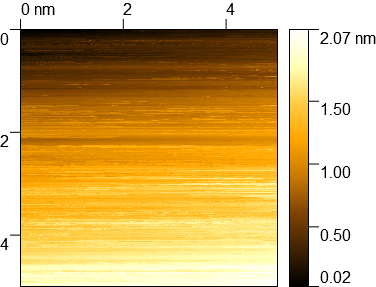
\includegraphics[width=\textwidth]{graphit_const_current_5nm_Z.png}
        %\label{fig:g_good_Z}
    \end{minipage}
    \caption{
      RTM-Aufnahme HOPG $\SI{5}{\nm}$; links: Tunnelstrom, rechts: Z-Achse; Setpoint $I = \SI{1}{\nano\ampere}$, Tip voltage $U = \SI{500}{\milli\volt}$,Rastergeschwindigkeit $v = \SI{16.8}{\nano\meter\per\second}$; $P = 1000$, $I = 2000$, $D = 0$
}
    \label{fig:5nmCC}
\end{figure}

\begin{figure}[H]
    \centering
    \begin{minipage}[t]{0.495\textwidth}
        \centering
        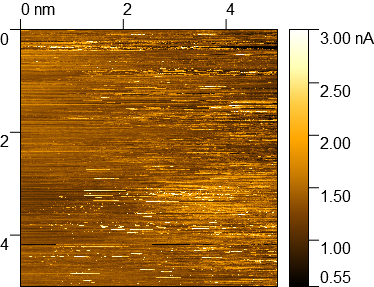
\includegraphics[width=\textwidth]{graphit_const_height_5nm_I.png}
        %\label{fig:g_good_I}
    \end{minipage}
    \hfill
    \begin{minipage}[t]{0.495\textwidth}
        \centering
        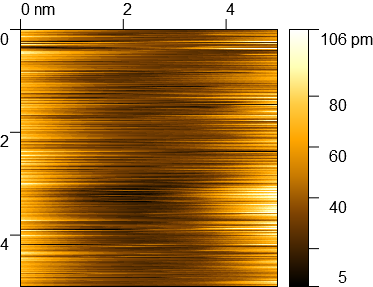
\includegraphics[width=\textwidth]{graphit_const_height_5nm_Z.png}
        %\label{fig:g_good_Z}
    \end{minipage}
    \caption{
      RTM-Aufnahme HOPG $\SI{5}{\nm}$; links: Tunnelstrom, rechts: Z-Achse; Setpoint $I = \SI{1}{\nano\ampere}$, Tip voltage $U = \SI{500}{\milli\volt}$,Rastergeschwindigkeit $v = \SI{16.8}{\nano\meter\per\second}$; $P = 0$, $I = 4$, $D = 0$
}
    \label{fig:5nmCH}
\end{figure}



Entgegen den Erwartungen zeigt die Strommessung in \cref{fig:5nmCH}keine klare periodische Struktur, die der Elektronendichte des Kristalls zugeschrieben werden könnte. 
Überraschenderweise sind einige helle und unregelmäßige Streifen sichtbar. Zur Korrektur dieses Fehlers wurden die Betriebsparameter variiert, um mögliche Störquellen durch unzureichende Scan-Geschwindigkeit oder andere Einflüsse auszuschließen. 
Die Messung wurde mehrfach neu gestartet, jedoch wurde keine erhebliche Verbesserung erzielt. Letztendlich erschien die beobachtete Struktur willkürlich und ungeordnet.

Alle verschiedenen Faktoren, vom ''Voltage'' bis zu ''Times per line'', vom Abziehen neuer Schichten der Graphitprobe bis zum Einsatz verschiedener Spitzen und sogar dem erneuten Starten des Experiments von Grund auf (einschließlich neuer Kalibrierung), führten nicht zu erwartungsgemäßen Ergebnissen.


Die nächste Annahme war, dass die Spitze zu stumpf und daher nicht atomar scharf sei, weshalb eine neue Spitze gezogen wurde. Selbst nach dem Austausch der Spitze war keine atomare Struktur zu beobachten.

Daher wurde vermutet, dass die Graphitprobe noch stark kontaminiert war und dass die verbleibenden großen Höhenunterschiede die Messung erheblich beeinflussten. Diese Abweichung könnte auf eine unebene Oberfläche hindeuten, obwohl später festgestellt wurde, dass dies wahrscheinlich nicht der Fall war. Tatsächlich liegt die tatsächliche Abweichung nur im Bereich weniger Nanometer, und die Farbskala wird durch einige Ausreißer verzerrt. Diese Ausreißer wurden höchstwahrscheinlich durch Schwankungen oder Rauschen verursacht.


Letztlich konnte die Messung im ''Constant Height Mode'' durchgeführt werden, ohne dass die Spitze in die Probe stürzte. Dennoch wurde die Probenoberfläche erneut frisch mit Klebeband abgezogen. Leider wurde aufgrund der Konzentration auf die genaue Fehlerquelle versäumt, Bilder von der neuen Probenoberfläche und der Spitze aufzunehmen.


Für die erneute Reinigung der Probenoberfläche musste der Probenhalter entfernt werden, wodurch die zuvor untersuchte Stelle verloren ging. Es musste ein neuer Bereich auf der Probe gefunden werden. Während dieser Versuche traten Probleme mit der Bewegung des Probenhalters auf. Die ''Approach''-Funktion konnte häufig nicht ausgeführt werden, da sich der Probenhalter trotz der Anzeige ''Moving'' im Programm nicht bewegte. Daher wurden stattdessen Versuche unternommen, sich der Probe mit den Funktionen ''Advance'' und ''Withdraw'' zu nähern. Dies führte dazu, dass die Spitze wiederholt in die Probe stürzte, was den Prozess erheblich verzögerte.
\clearpage
\subsection*{Fehleranalyse}
Das nicht gelungene Erreichen der atomaren Auflösung in diesem Experiment ist unerwünscht, aber nicht ausgeschlossen. Daher existieren mehrere Fehlerquellen, die in diesem Abschnitt untersucht werden.


Zunächst spielt die Qualität der Spitze eine wesentliche Rolle für den Erfolg dieses Experiments. Wie bereits erläutert, gestaltete es sich aufgrund zittriger Hände allgemein schwierig, scharfe, hochwertige Spitzen herzustellen.
Das Versagen des Probenhalters führte außerdem häufig dazu, dass die Spitze in die Probe stürzte, wodurch ihre Qualität weiter beeinträchtigt wurde. Eine Multiatomspitze verringert die Tunnelingwahrscheinlichkeit von Elektronen erheblich, da sie nicht mehr als mikroskopisches System betrachtet werden kann.


Es ist jedoch unwahrscheinlich, dass die Spitze die primäre Fehlerquelle war. Es ist wichtig zu beachten, dass in allen Messungen durchgehend ein Tunnelstrom beobachtet wurde, was die Möglichkeit einer makroskopisch stumpfen Spitze ausschließt. Darüber hinaus wurde die Spitze mehrfach ausgetauscht.


Eine weitere theoretische Fehlerquelle könnte die raue Oberfläche der Graphitprobe sein. Diese Fehlerquelle kann jedoch als vernachlässigbar angesehen werden, da die Oberfläche während der zweiten Messung sorgfältig abgezogen wurde und alle Messungen konsequent auf glatten Bereichen durchgeführt wurden.


Störungen wie Vibrationen durch mechanische Bewegung, Schallwellen oder elektrisches Rauschen können als Fehlerquellen ausgeschlossen werden. Solche Einflüsse würden die Ergebnisse nur geringfügig verzerren und sie nicht vollständig ungültig machen.

Ein Faktor, der einen erheblichen Einfluss auf die Beobachtung und Analyse der HOPG-Struktur haben kann, ist die unzuverlässige Funktionalität der ''Approach''- und ''Withdraw''-Funktionen, da es mehrfach vorkam, dass der Status der Spitzen-Proben-Verbindung während eines einfachen Versuchs abbrach oder instabil wurde und der Kalibrierungsprozess vollständig wiederholt werden musste. Dies würde mit Sicherheit zu einer unebenen Oberfläche führen und somit die Identifikation einer geordneten Struktur zusätzlich erschweren.


Von den erörterten Fehlerquellen erscheint Letztere im Hinblick auf ihre potenziellen Auswirkungen auf die Messdaten als die plausibelste. Dennoch könnten auch die anderen Fehlerquellen eine wesentliche Rolle beim erfolglosen Erreichen der atomaren Auflösung gespielt haben.


Um die Wahrscheinlichkeit zu erhöhen, in zukünftigen STM-Experimenten eine atomare Auflösung zu erzielen, ist ein kontrollierterer und systematischerer Ansatz bei der Spitzenvorbereitung unerlässlich. 
Obwohl während des Experiments mehrere Spitzen verwendet wurden, führte die Herstellungs- und Handhabungsmethode zu Variabilität, die die Leistungsfähigkeit beeinträchtigt haben könnte. 
Bei nachfolgenden Versuchen könnte der Einsatz von vorab geschärften kommerziellen Spitzen (z. B. geätzte Pt/Ir- oder W-Spitzen mit bekanntem Spitzenradius < $\SI{10}{\nm}$) Konsistenz gewährleisten und Vorbereitungsfehler verringern. 
Darüber hinaus könnten in situ-Konditionierungs\-techniken - wie kontrollierte Feldelektronenemission oder sanftes Spannungspulsen über sauberem Gold - die Spitzenflächenschärfe verbessern und Kontamination an der Spitze verringern, was für die Auflösung des atomaren Gitters entscheidend ist.

Ein weiterer entscheidender Verbesserungsbereich liegt in der Parameteroptimierung und in Echtzeitdiagnosen während des Scans. Rückblickend wäre es vorteilhaft gewesen, einen systematischen Scan-Parameter-Überblick durchzuführen - dabei Bias-Spannung, Sollstrom, Scan-Geschwindigkeit und PID-Verstärkungsfaktoren zu variieren -, um den Bereich zu identifizieren, der die atomare Auflösung am besten begünstigt. 
Beispielsweise könnte durch eine Verringerung des Scan-Gebiets auf unter $\SI{10}{\nm}$ bei gleichzeitiger Erhöhung der Pixeldichte und einer vorsichtigen Anhebung des Sollstroms eine bessere Auflösung feiner Oberflächenstrukturen erzielt werden. Der Einsatz von Testproben mit gut charakterisierten atomaren Gittern (z. B. frisch präpariertes Au(111)) als Referenz könnte zudem dabei helfen, die Einstellungen zu optimieren, bevor auf HOPG umgeschaltet wird, und so den Abbildungsprozess robuster gestalten.

Schließlich können erhebliche Verbesserungen durch die Erhöhung der mechanischen und elektronischen Stabilität erzielt werden. Die Instabilität des groben Heranfahrmechanismus und die unzuverlässige Spitzen-Proben-Kopplung haben wahrscheinlich Drift und abrupte Änderungen der Spitzenhöhe verursacht, was die Konsistenz der Feinscans untergrub. 
Falls verfügbar, würde die Integration automatisierter Heranfahrmechanismen mit ''Closed-Loop-Feedback'' diese Probleme entschärfen. Darüber hinaus würde das Sicherstellen längerer Gleichgewichtszeiten nach jedem Heranfahrzyklus sowie die Minimierung akustischer und thermischer Schwankungen in der Laborumgebung die Positionsdrift während des Scans verringern. 
Zusammen würden diese Verfeinerungen eine stabilere und kontrolliertere experimentelle Bedingung schaffen, unter der atomare Auflösung zuverlässiger erreicht wird.

Abschließend kann festgehalten werden, dass - obwohl die angewandten Methoden in diesem Versuch keine atomare Auflösung erzielten - das Experiment dennoch eindrucksvoll verdeutlichte, wie empfindlich STM-Messungen auf geringfügige Veränderungen in Aufbau und Durchführung reagieren. 
Von den Schwierigkeiten beim Grobheranführen und der Spitzenstabilität bis hin zur Abstimmung der Scan-Parameter wird offensichtlich, dass kleine Unachtsamkeiten schnell zu einem Auflösungsverlust führen können. 
Zugleich ergibt sich nun ein wesentlich klareres Bild dessen, worauf bei künftigen Versuchen besonders geachtet werden muss - insbesondere in Bezug auf Rückkopplungsregelung, Spitzenkonditionierung und Probenvorbereitung. 
Mit einem sorgfältigeren und konsistenteren Vorgehen sollte das Erfassen des atomaren Gitters definitiv möglich sein.

